%%%%%%%%%%%%%%%%%%%%%%%%%%%%%%%%%%%%%%%%%%%%%%%%%%%%%%%%%%%%
% Template prepared by Dr Daniel Oi, CC BY-NC 4.0          %
%%%%%%%%%%%%%%%%Do Not Alter The Preamble%%%%%%%%%%%%%%%%%%%

%%%%%%%%%%%%%%% Preamble Starts Here %%%%%%%%%%%%%%%%%%%%%%%
%
\documentclass[aps,pra,a4paper,nofootinbib,onecolumn,tightenlines,longbibliography,12pt,amsfonts,amssymb,amsmath,floatfix]{revtex4-2} % Uses the APS RevTeX document class. Versions earlier than 4-2e may not be compatible with the latest LaTeX kernel.
\usepackage{latexsym,graphicx,color,geometry}
\geometry{a4paper, portrait, hmargin=2cm, vmargin={2cm, 2.5cm}}%Defines the page size and margins
\usepackage{url}%Fixes URLs in bibliography
\usepackage{enumitem}%Numbering in Lists
\usepackage[english]{isodate,babel}
\usepackage[figure,table]{totalcount} % counts tables and figures
\usepackage{blindtext} % used to make some example junk text
\usepackage{physics} % very useful for typesetting physics equations
\usepackage{float}
\def\bibsection{\section*{\refname}} %Sorts out reference section and gets rid of horizontal line
\bibliographystyle{acm}
\usepackage{titlesec}
\titleformat*{\section}{\Large\bfseries}
\titleformat*{\subsection}{\large\bfseries}
\titleformat*{\subsubsection}{\normalsize\bfseries\itshape}
\titleformat*{\paragraph}{\large\bfseries}
\titleformat*{\subparagraph}{\large\bfseries}

%%%%Font Definition%%%%
% the document is to be sans serif
\usepackage[T1]{fontenc}
%\usepackage[cmbright]{sfmath}
\usepackage{lmodern}
\renewcommand{\rmdefault}{lmss}
\renewcommand{\sfdefault}{lmss}
\renewcommand{\mathbf}[1]{\ensuremath\textbf{\textit{\textsf{#1}}}}

%%%%%%%%%%%%%%%%%%% Preamble Ends Here %%%%%%%%%%%%%%%%%%%%%%%%


%%%%%%%%%%%%%%%%%%%%%%%%%%%%%%%%%%%%%%%%%%%%%%%%%%%%%%%%%%%%%%%
% Insert any other extra packages or definitions you want here%


%                                                             %
%%%%%%%%%%%%%%%%%%%%%%%%%%%%%%%%%%%%%%%%%%%%%%%%%%%%%%%%%%%%%%%


%%%%%%%%% Fill in your details in the part below %%%%%%%%%
\newcommand{\projecttitle}{Evaluating Spot Finding Methods}% Change title and remove red text color
\newcommand{\studentname}{Anton Gashi}% Type in your name here, but without the red highlighting, same for all other uses of red text
\newcommand{\regnumber}{201914462}
\newcommand{\degree}{MPhys}
\newcommand{\primarysup}{Dr Sebastian Van De Linde}
\newcommand{\secondsup}{Dr Daniel Oi}%Comment out this line if not needed
%\newcommand{\thirdsup}{\textcolor{red}{Dr~C~Bloggs}}%Comment out this line if not needed
%%%%%%%%%%%%%%%%%%%%%%%%%%%%%%%%%%%%%%%%%%%%%%



%%%%% Do Not Alter this part %%%%%%%%%%%%
\usepackage{fancyhdr}
\pagestyle{fancy}
\setlength{\headheight}{14pt}
\footskip = 45pt
\fancyhf{}
\lhead{\projecttitle} 
\lfoot{PH450 Report 2021-22}
\cfoot{Student: \regnumber}
\rfoot{Page \thepage}
%%%%%%%%%%%%%%%%%%%%%%%%%%%%%%%%%%%%%%%%%


%%%%%%The document starts here%%%%%%
\begin{document}

%%This section creates the cover page%%

\begin{figure}

\includegraphics[width=\textwidth]{ScienceLogo.png}
\end{figure}

\title{PH450 Report 2021-22\\ \vspace{1cm}
{\huge \projecttitle}\\[0.5cm] %If your title is too long, use \LARGE, \Large, or large instead of \huge
{\footnotesize Submitted in partial fulfilment for the degree of \degree}}

\author{\studentname\\
Registration No.: \regnumber}
\affiliation{SUPA Department of Physics, University of Strathclyde, Glasgow G4 0NG, United Kingdom}

\author{\primarysup{} (Primary Supervisor)}
\noaffiliation
\ifdefined\secondsup % this only appears if \secondsup is set above
\author{\secondsup, (Secondary Supervisor)} % 
\noaffiliation
\fi
\ifdefined\thirdsup
\author{\thirdsup, (Secondary Supervisor)} % 
\noaffiliation
\fi

\date{\today}

\pagenumbering{gobble} % first page in document is not numbered

\maketitle
%%This ends the title page section%%

\newpage % Creates a new page

\pagenumbering{roman} %Use Roman numerals for the front matter pages

\section*{Abstract} %The * suppresses a section number
\addcontentsline{toc}{section}{Abstract}

\newpage
\section*{Acknowledgements}
\addcontentsline{toc}{section}{Acknowledgements}


%%%%%%%%%%%%%%%%%%%%%%%%%%%%%
% Do not alter this section %
\newpage
\tableofcontents % Creates a Table of Contents
\makeatletter
\let\toc@pre\relax
\let\toc@post\relax
\makeatother

\ifnum\totalfigures>0
\newpage
\listoffigures
\addcontentsline{toc}{section}{List of Figures}
\fi

\ifnum\totaltables>0
\newpage
\listoftables
\addcontentsline{toc}{section}{List of Tables}
\fi


% Can edit after here       %
%%%%%%%%%%%%%%%%%%%%%%%%%%%%%


%%%%% Main Report Starts Here %%%%%

\newpage
\pagenumbering{arabic}

\section{Introduction}

  \subsection{Sub-Pixel Localisation} % (fold)
  \label{sub:spot-finding intro}
  
  Super-resolution microscopy is the process of taking the diffraction limit 
  of a microscope, ~250nm in the x and y direction, and improving it by a 
  factor of 2. In the past this has been achieved by ensemble techniques
  like SIM (Structured Illumination Microscopy) and STED (Stimulated Emission Depletion)
  \textbf{insert explanation of ensemble techniques}. An improvement on these methods 
  is single-molecule microscopy, in which whatever is being imaged overcomes the 
  diffraction limit by being fluorescent. This helps as the fluorescence emits the light 
  stochastically so only a subset of molecules "light-up" at once, this is important 
  as if they are separated by at least 200nm then they can be located to nanometre precision. 
  Since the molecules are now separated spatially you just need to repeat this process temporally
  until all molecules have been "switched-on", this gives a stack of images with blurry spots
  which can be located and recombined into a final image with spot-precision on the order of ~20nm.\cite{galbraith2011super}
  The resolution of a super-resolution image usually doesn't refer to the spot-precision of the 
  located molecule, rather it refers to the structural resolution, this can be calculated along 
  with the density of fluorophores as the Nyquist-Shannon sampling theorem states a minimum number 
  of fluorophores are required to resolve the structure. For example if the resolution is 20nm in 
  one dimension then fluorophores have to be separated at least 10nm apart at a density of 
  $~10^4\mu m^{-2}$.\cite{van2011single}\cite{shannon1949communication}

  
  \subsection{reasoning behind my project} % (fold)
  \label{sub:reasoning behind my project}
  
  The main motivation behind my project is to improve the compute time that it
  takes to render images through sub-pixel localisation whilst keeping an
  acceptable level of accuracy. That is to say this project should be aiming to
  produce a method of spot-finding that either less complex, less computations
  per localisation, fewer steps or a mixture of all.

  \textbf{
  With the almost exponentially increasing launching of small form factor
  satellites such as the CubeSat, arises the challenge of efficiently utilising
  the satellites computing resources. This means any segment of code being ran on
  the satellite needs to run as quickly as possible whilst keeping a certain
  standard of accuracy, especially for the processes that the satellite depends
  on to operate like attitude control, power management and calculations for
  orbital maneuvers. The main method used for orienting(attitude control) CubSat
  like satellites is by using a Star Tracker, this work by using a camera mounted
  facing stars that are known to the satellite via a star catalogue and moves
  based on how aligned or unaligned a reference image is with the actual image
  seen.\cite{calitz2015design} The method in which the image is processed so it
  can be compared to the reference is called spot finding, this entails taking
  the image and finding each bright spot or star accurately. The motivation for
  this project is to develop a spot finding method for star tracking and compare
  it to the state of the art algorithms measuring accuracy, precision and speed.}
  \textbf{
  This technique is also used for super-resolution microscopy, which changes the
  optical limits of microscopy from 250nm to about 10nm, this is achieved by
  temporally or spatially spacing the light coming from the specimen being
  imaged. There are two ways of doing this photo-activated localization
  microscopy(PALM) and stochastic optical reconstruction microscopy(STORM), both
  rely on fluorophores which are fluorescent chemicals that re-emit light after
  being excited but they also emit the light stochastically so with a fast enough
  camera the light spots can be independently seen. This also requires a method
  of finding and recombining each spot in each frame to obtain a final sharper
  image than before.\cite{small2014fluorophore}}
  
  

% subsection subsection name (end)


\section{State of the field/lit review} % (fold)
\label{sec:State of the field/lit review}


The field of spot finding or star finding is a fairly recent field with papers
coming out in the mid 80's from NASA. However the methods haven't changed that
much since the main algorithm still used is centroiding since it's a very good
compromise between quickness and accuracy being that it can give an answer in
the 1-100 microsecond range \cite{delabie2014accurate}. Much of the innovation
has come from optimising the algorithm or optimising the data going into the
algorithm, in a 2011 paper by Zhai et al\cite{zhai2011micro} Nyquist sampling
was used to reconstruct an accurate point spread function(PSF) which helped
achieve micro-pixel accuracy.


\section{Methods} % (fold)
\label{sec:Background}

  \subsection{Centroiding} % (fold)
  \label{sub:Centroiding_meth}
  
  % subsection subsection name (end)
  
  
  The most common way of spot finding for star tracking is to use centroiding
  algorithms, this is when a subsection of pixels are considered to be a star
  using a rough calculation. The area of interest is then filtered in such a way
  that reduces noise and aberrations, finally apply the algorithm in this case
  it's the center of gravity method (\ref{eq1})(or the moment
  method)\cite{delabie2014accurate}\cite{stone1989comparison}.
  \begin{equation}\label{eq1}
      (x_b,y_b) = \left( {\frac{\sum_{ij} I_{ij}x_{ij}}{\sum_{ij} I_{ij}},\frac{\sum_{ij} I_{ij}y_{ij}}{\sum_{ij} I_{ij}}}\right)
  \end{equation}
  
  A powerful tool for image processing is ImageJ, this is an open source tool
  that can be used for anything from noise reduction, fourier transforms and
  finding maxima to analysis such as histograms to visualisations. 
  Even better because it's open source you can either find plugins or create one.
  \cite{van2019single}
  
    \begin{figure}[H]
      \begin{center}
        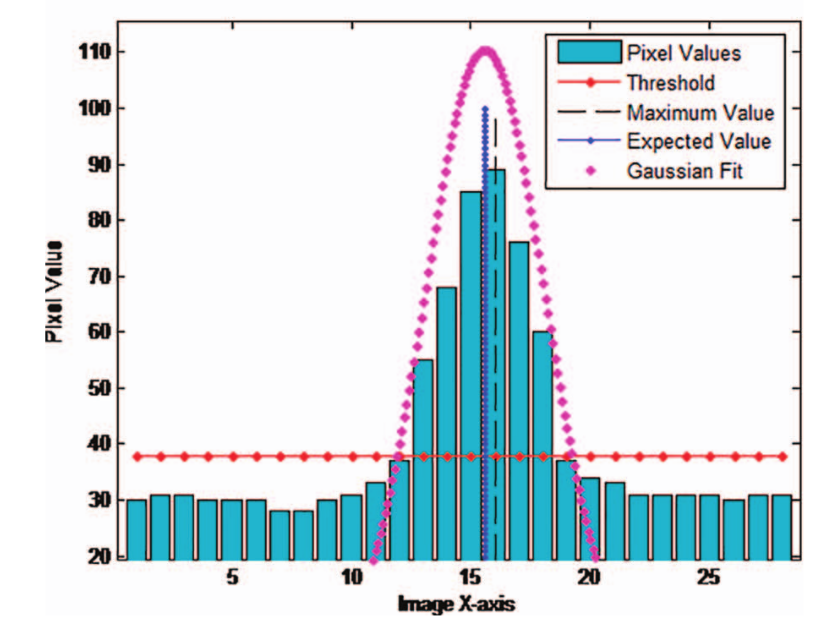
\includegraphics[width=0.5\textwidth]{litreview.png}
      \end{center}
      \caption{Intensity of real star data (Gienah) showing visually how data is pruned. \cite{rawashdeh2014image}}
      \label{fig:1}
    \end{figure}
  
  
  \subsection{Various fitting methods} % (fold)
  \label{sub:Various fitting methods}
  
    \subsubsection{Gaussian} % (fold)
    \label{ssub:Gaussian}


    
    \subsubsection{Triangular method} % (fold)
    \label{ssub:Triangular method}
  


\section{Theory (probably don't need)} % (fold)
\label{sec:Theory}

% section section name (end)


\section{Results} % (fold)
\label{sec:Results}

  \subsection{Centroiding} % (fold)
  \label{sub:Centroiding_results}
  
  \subsection{Triangle Fitting} % (fold)
  \label{sub:Triangle Fitting}
  
    \begin{figure}[H]
      \begin{center}
        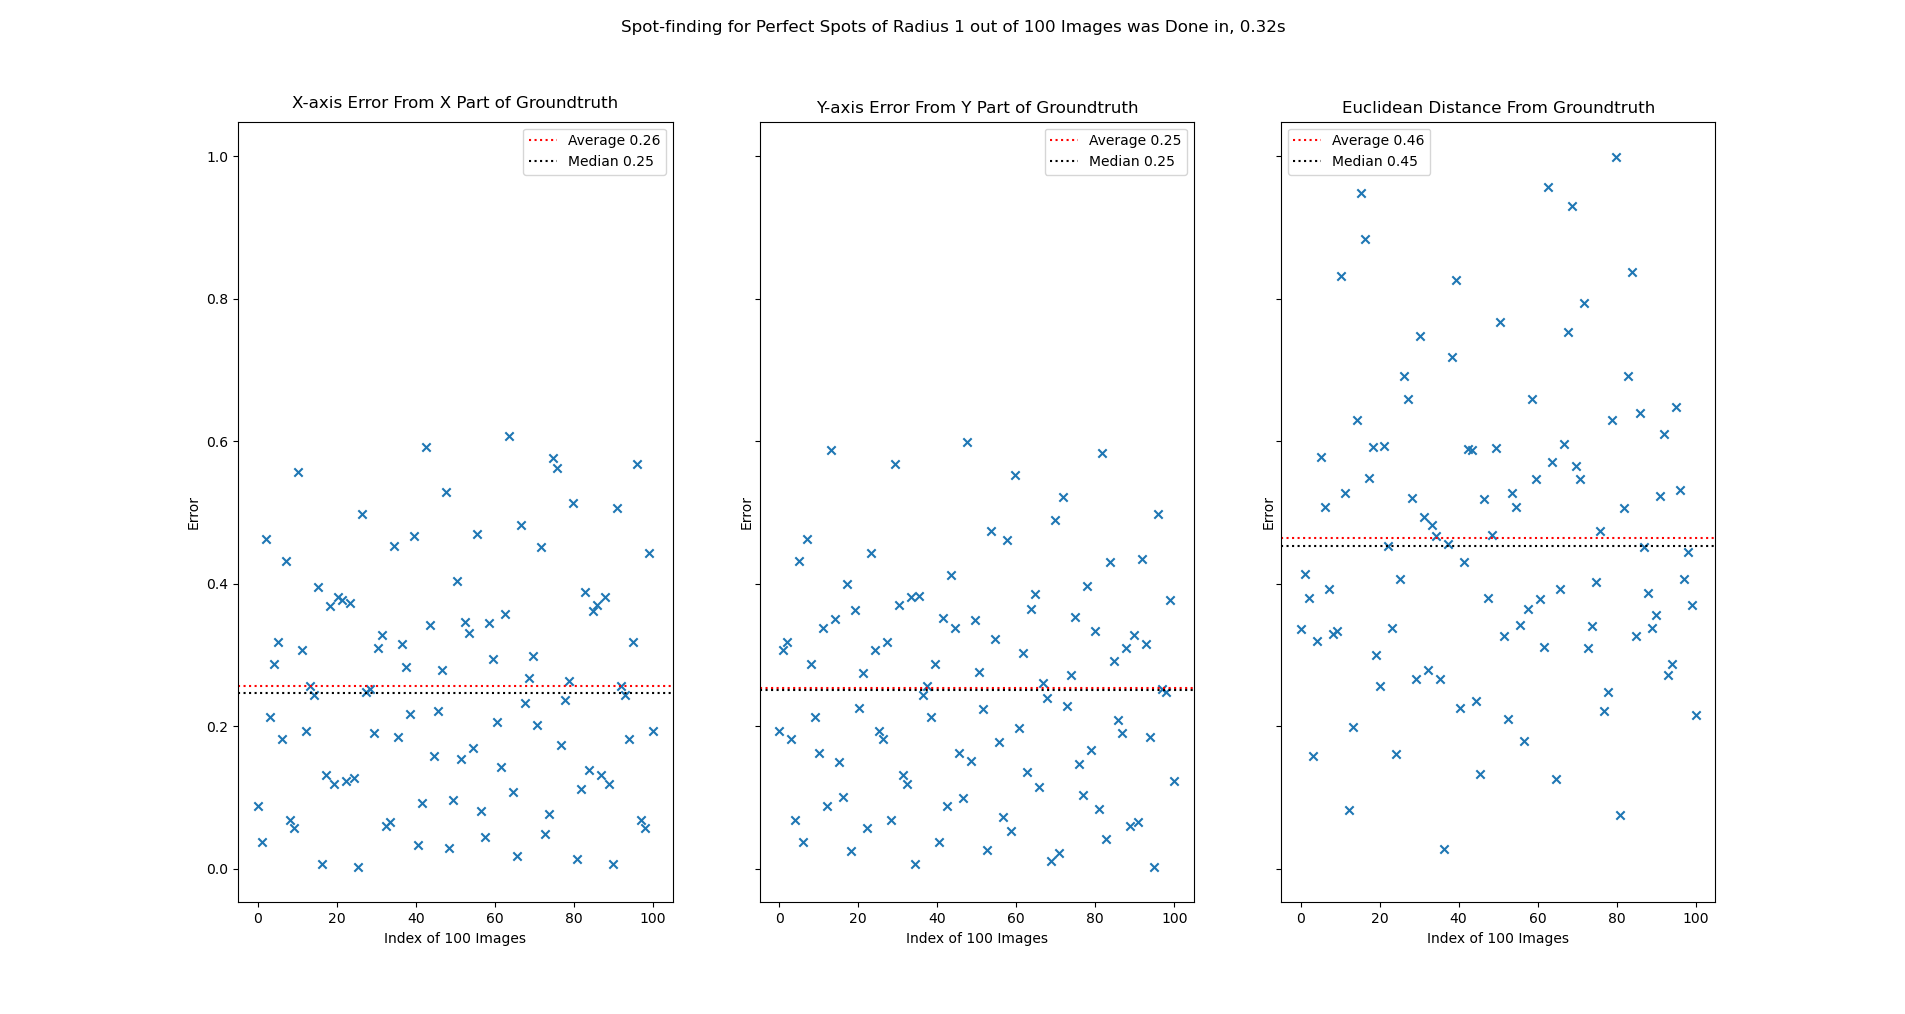
\includegraphics[width=1.0\textwidth]{project_pics/error_r1.png}
      \end{center}
      \caption{}
      \label{fig:tri_er_r1}
    \end{figure}
    
    \begin{figure}[H]
      \begin{center}
        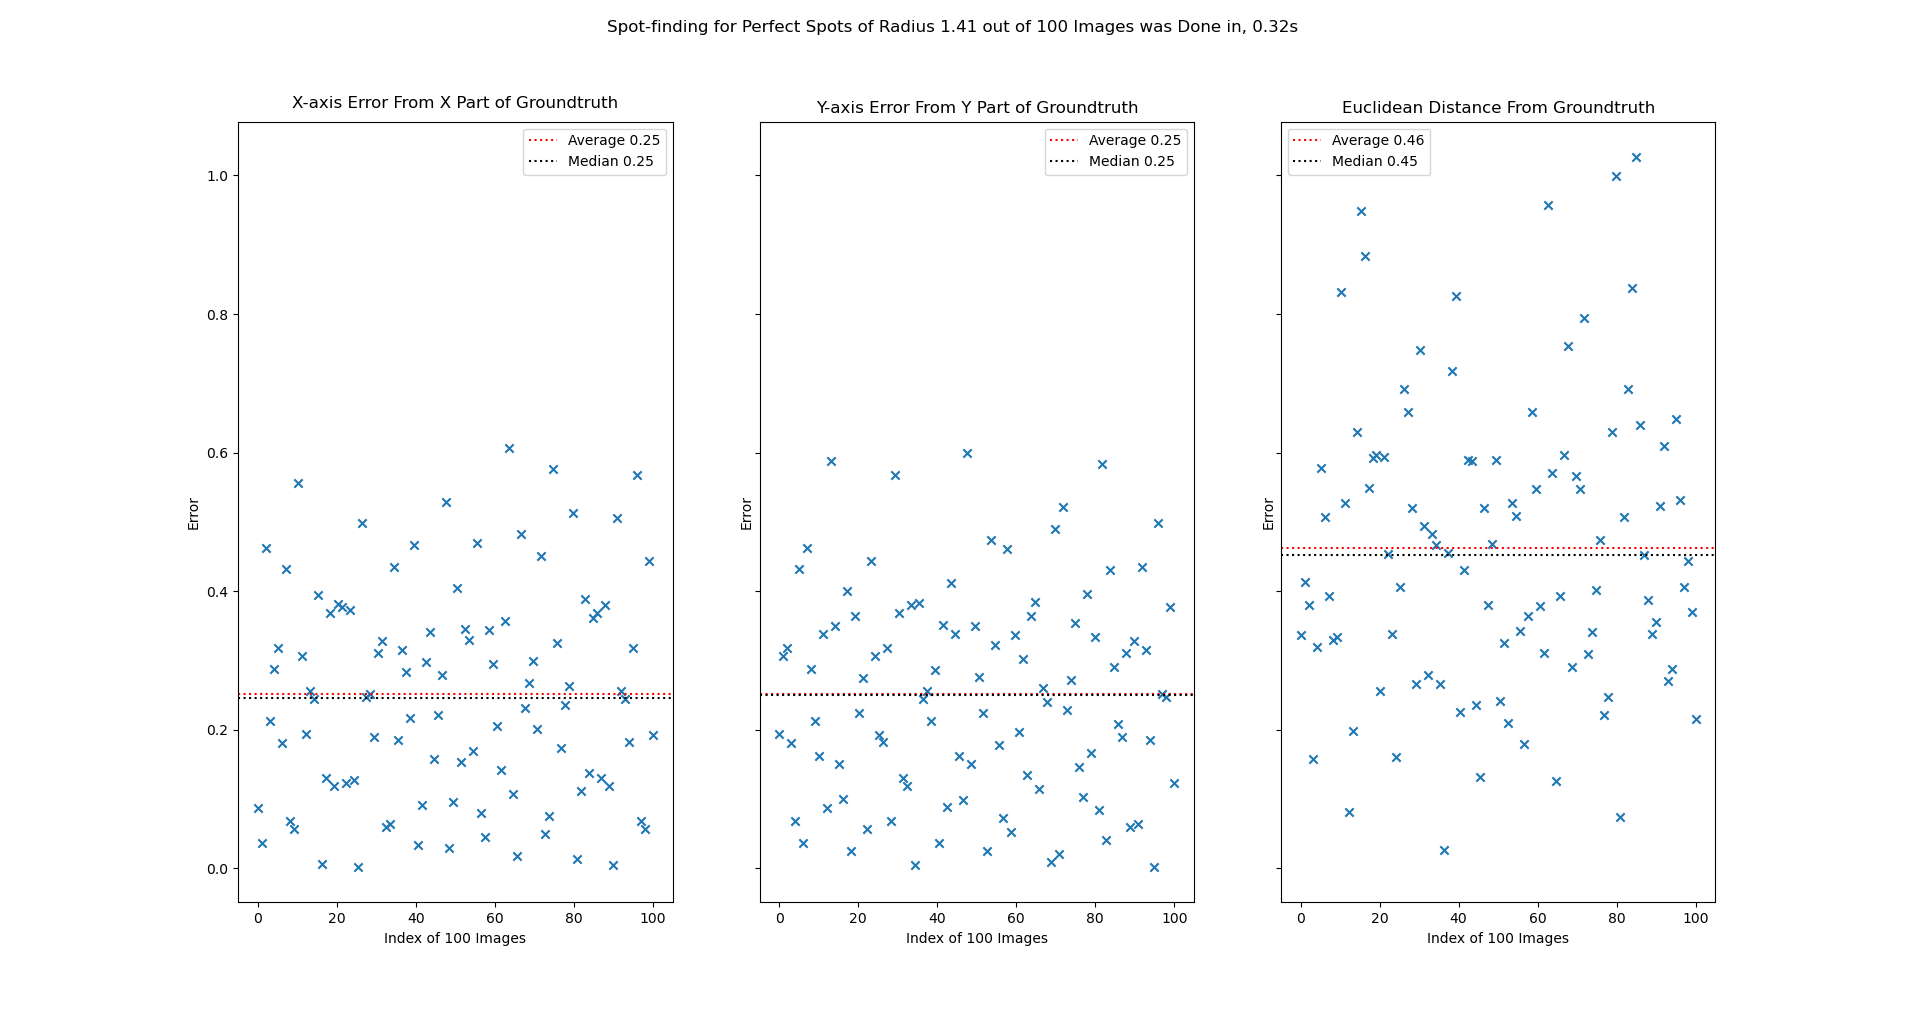
\includegraphics[width=1.0\textwidth]{project_pics/error_r141.png}
      \end{center}
      \caption{}
      \label{fig:tri_er_r141}
    \end{figure}
    
    \begin{figure}[H]
      \begin{center}
        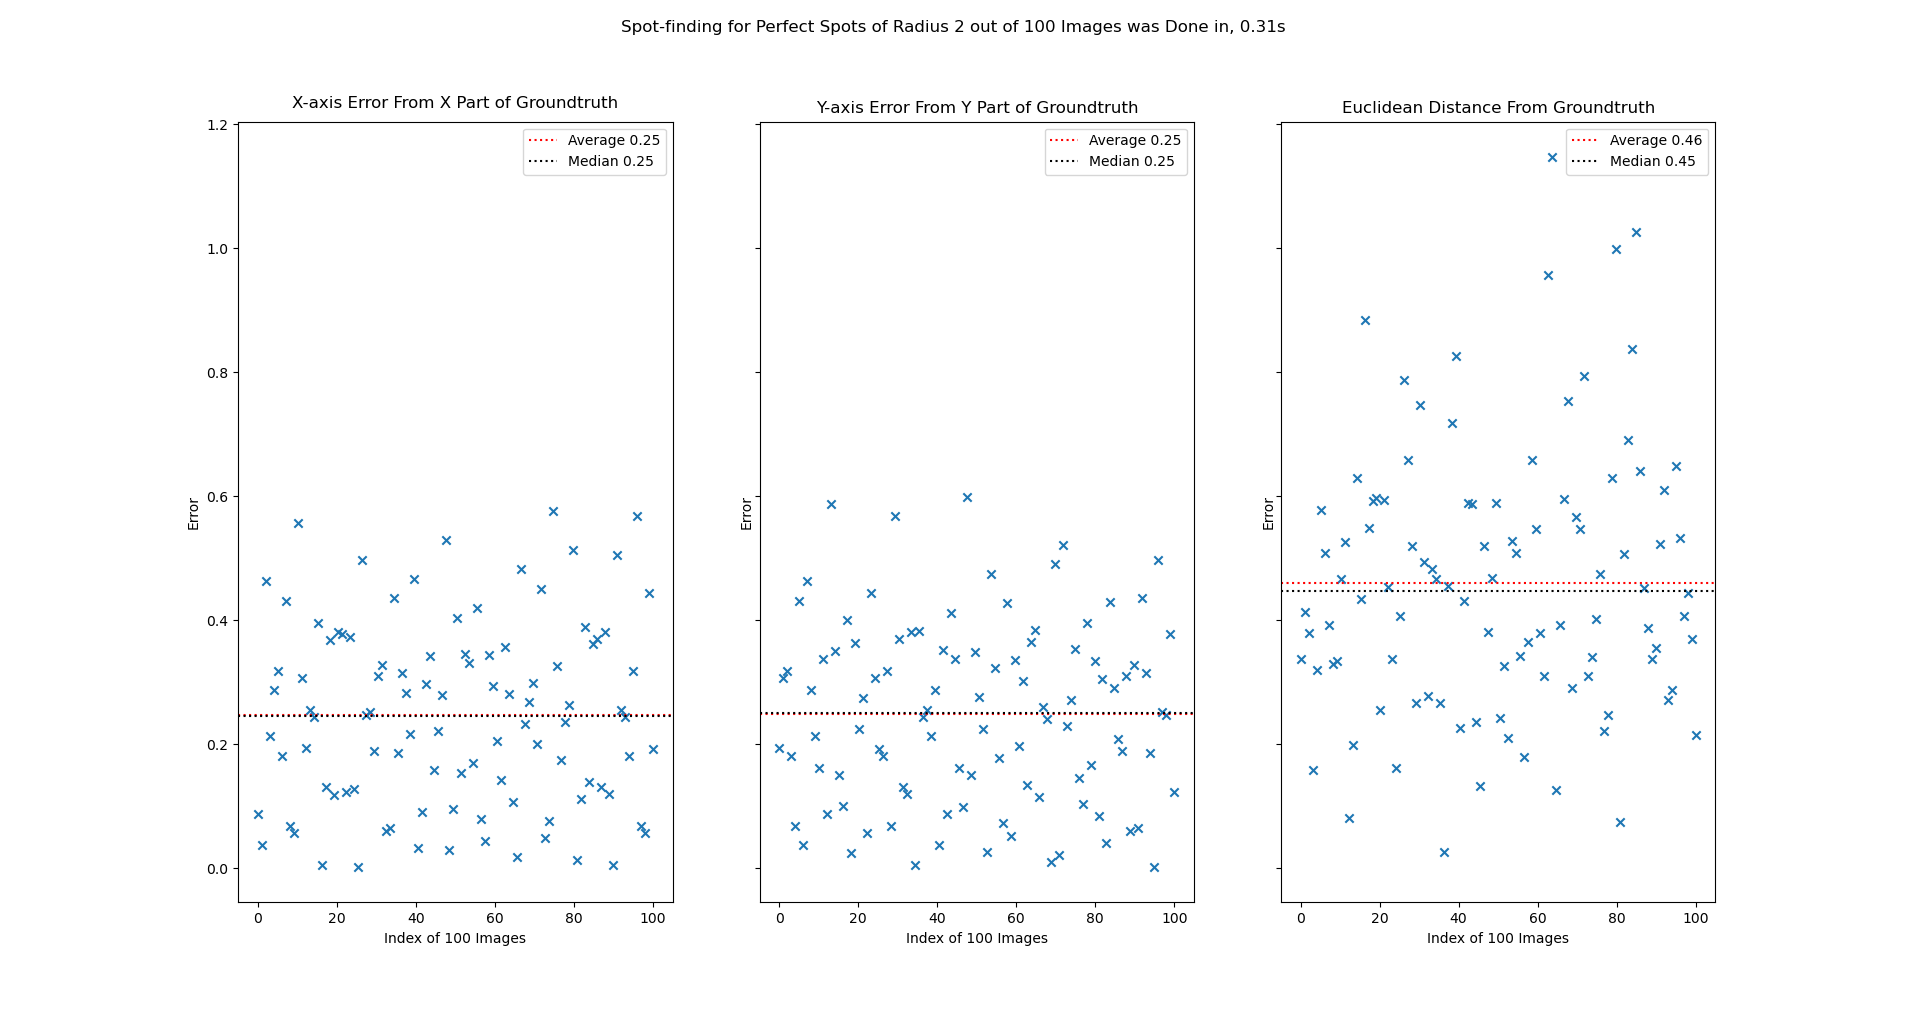
\includegraphics[width=1.0\textwidth]{project_pics/error_r2.png}
      \end{center}
      \caption{}
      \label{fig:tri_er_r2}
    \end{figure}
    
    \begin{figure}[H]
      \begin{center}
        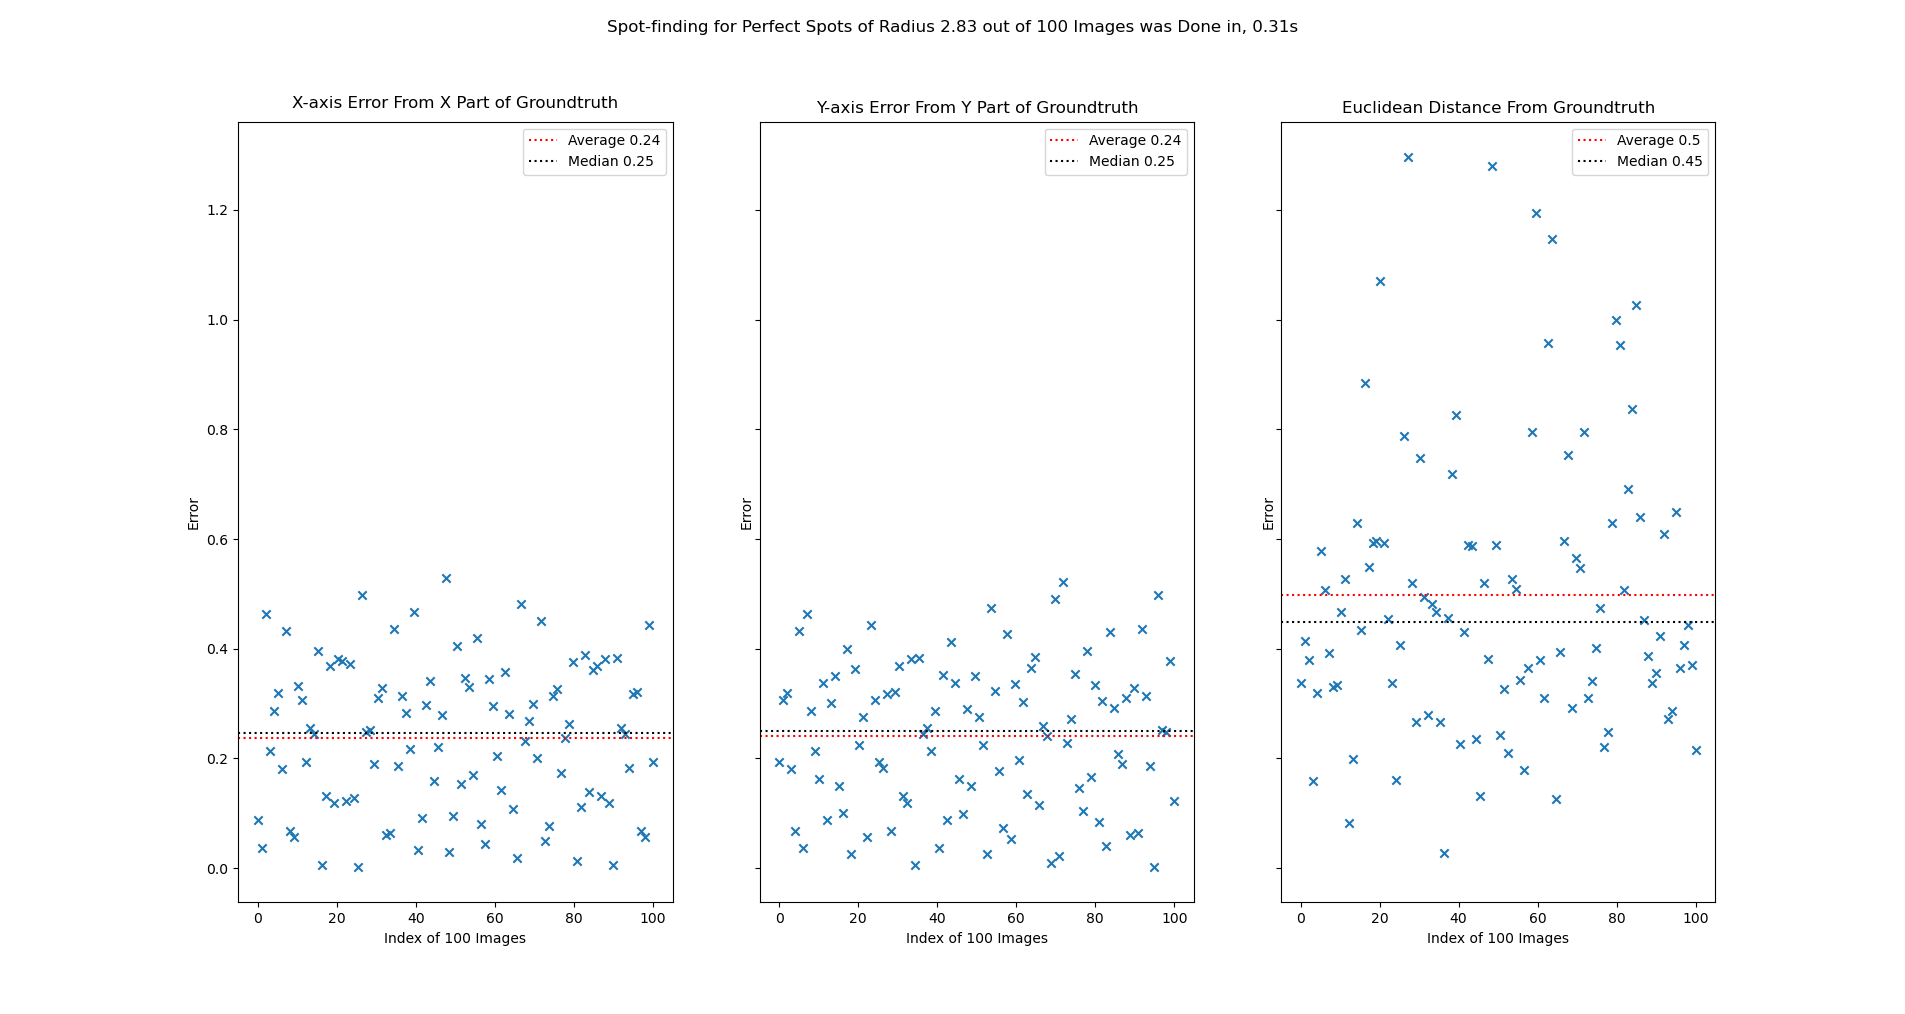
\includegraphics[width=1.0\textwidth]{project_pics/error_r283.png}
      \end{center}
      \caption{}
      \label{fig:tri_er_r283}
    \end{figure}
    
    \begin{figure}[H]
      \begin{center}
        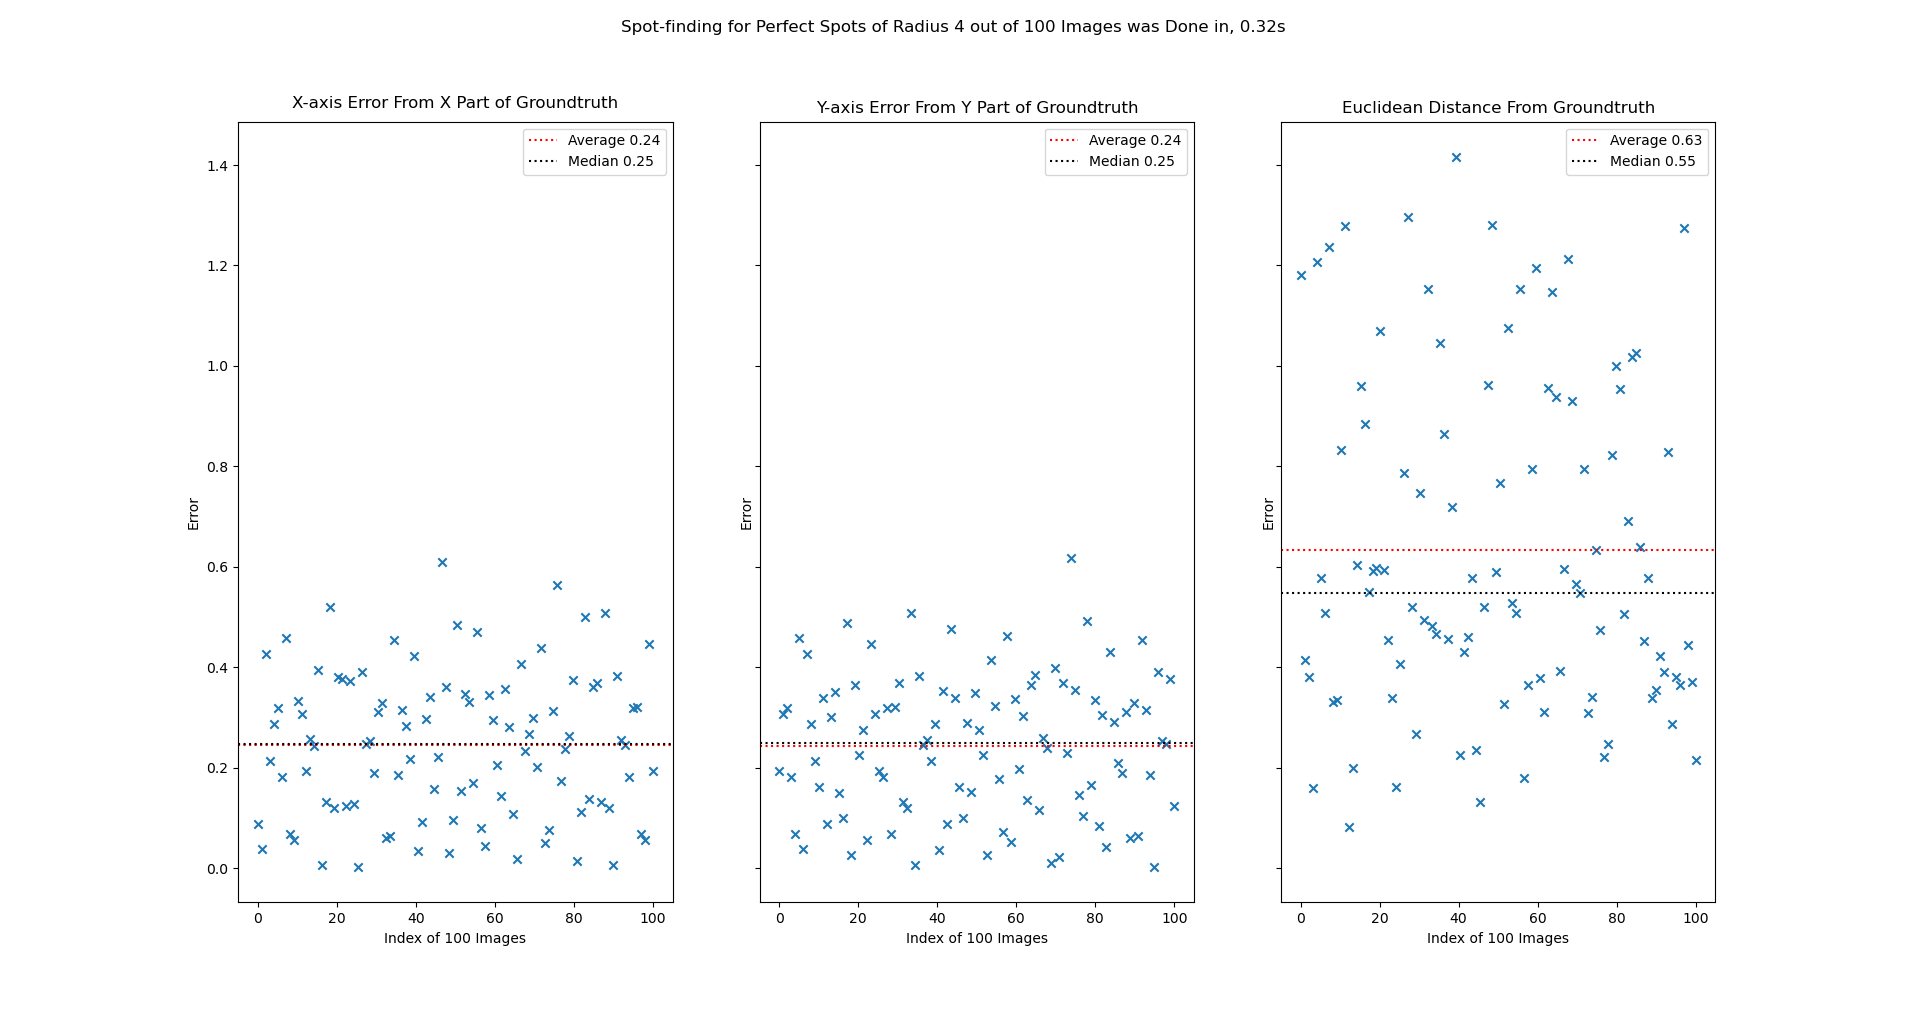
\includegraphics[width=1.0\textwidth]{project_pics/error_r4.png}
      \end{center}
      \caption{}
      \label{fig:tri_er_r4}
    \end{figure}
    
    \begin{figure}[H]
      \begin{center}
        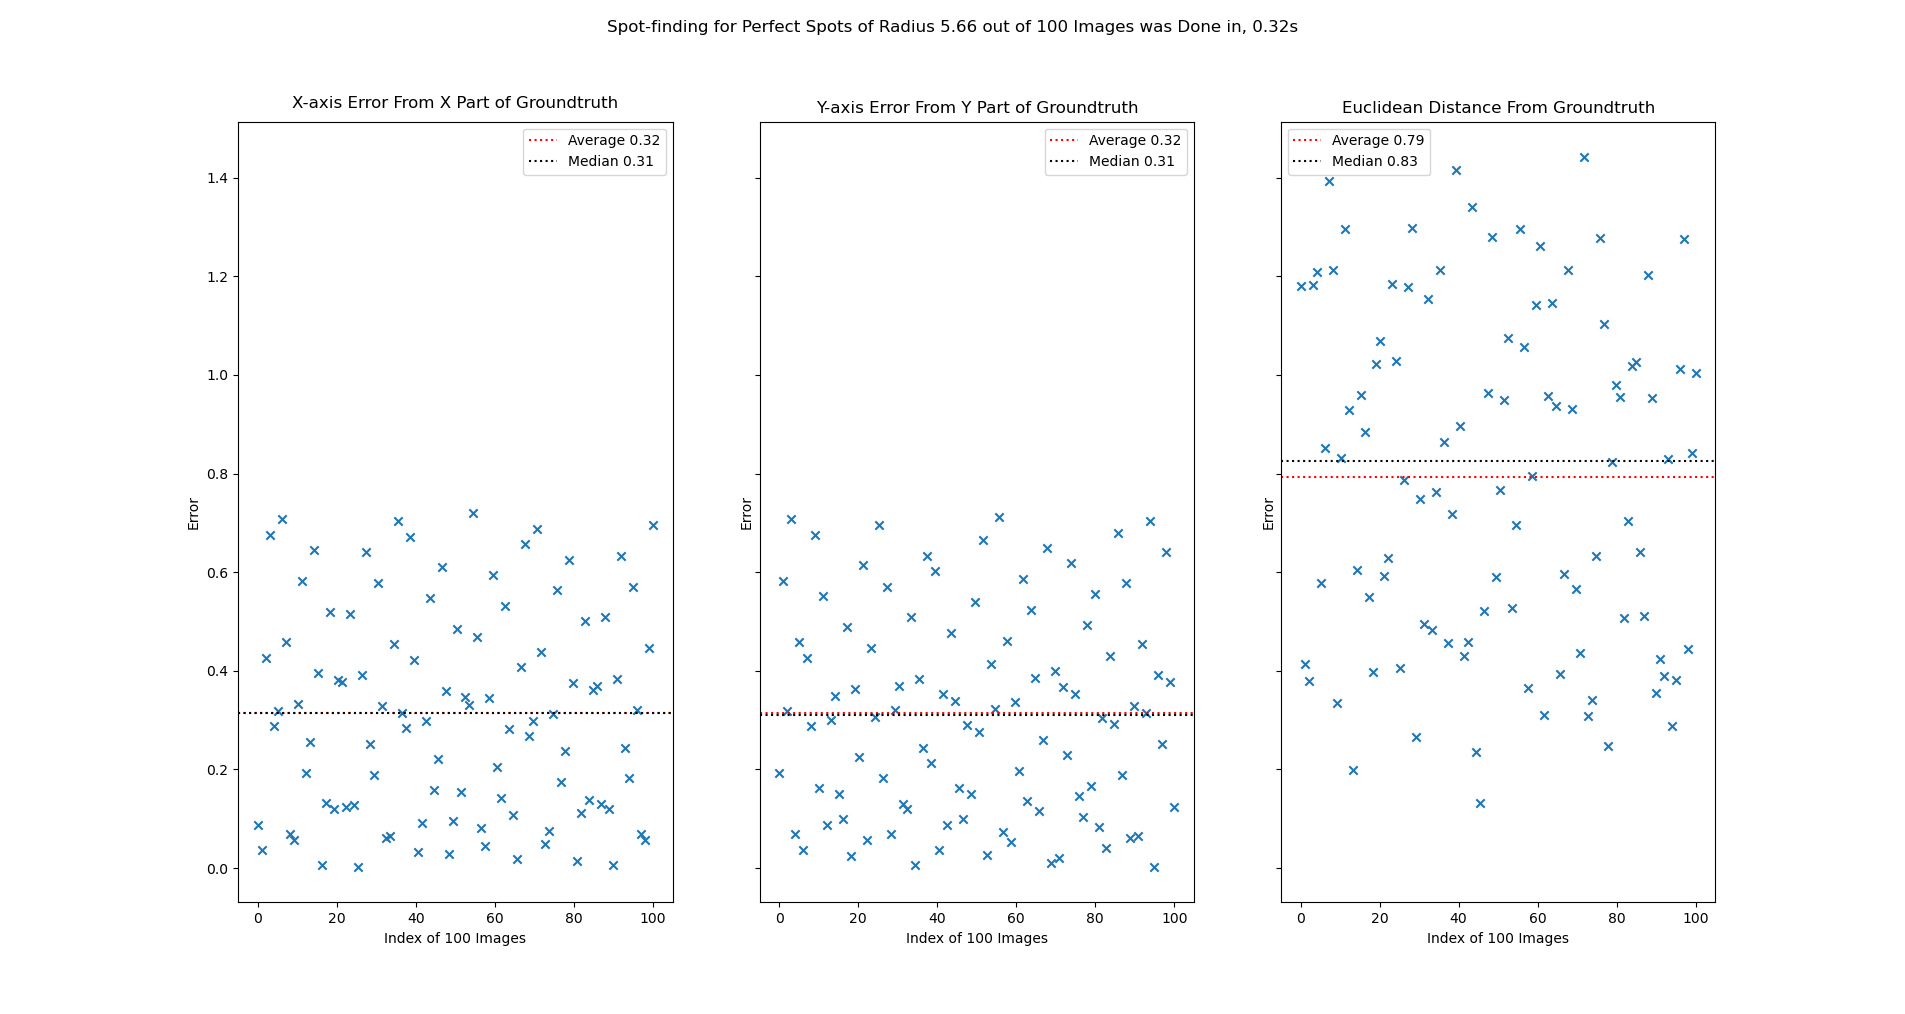
\includegraphics[width=1.0\textwidth]{project_pics/error_r566.png}
      \end{center}
      \caption{}
      \label{fig:tri_er_r566}
    \end{figure}
    
    \begin{figure}[H]
      \begin{center}
        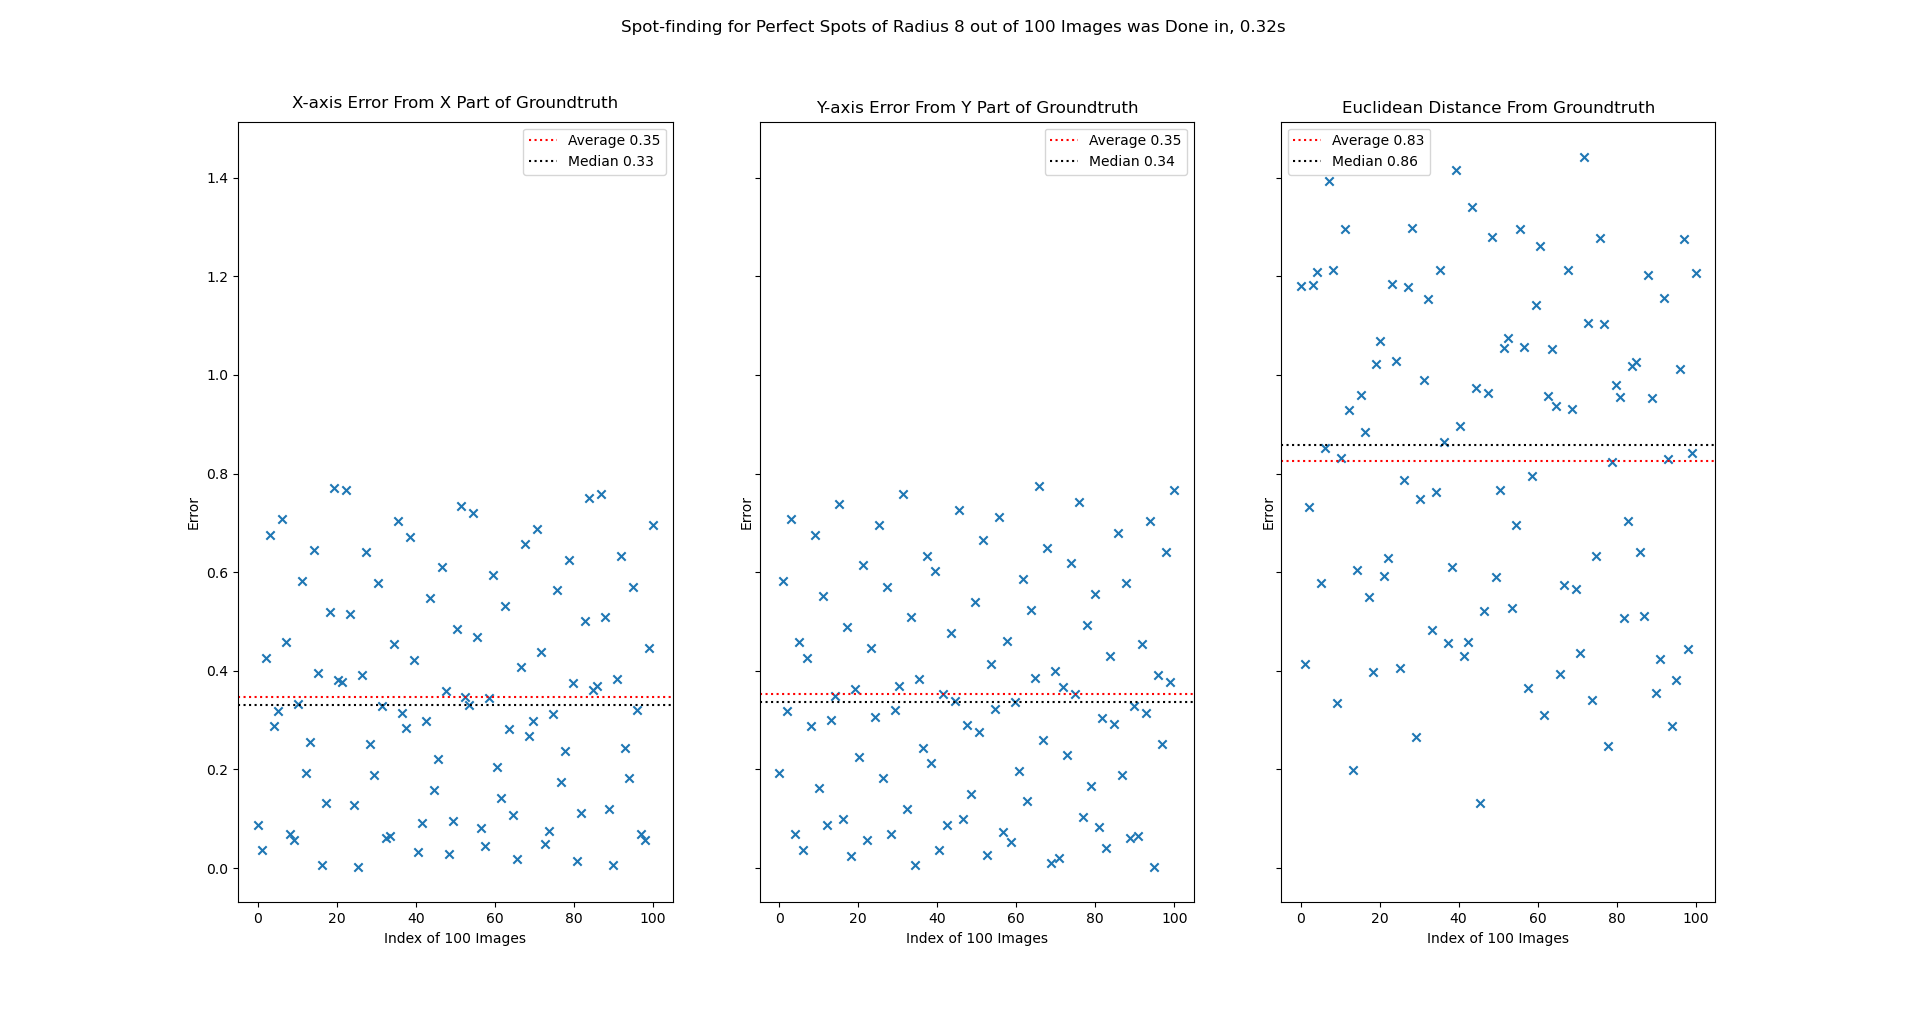
\includegraphics[width=1.0\textwidth]{project_pics/error_r8.png}
      \end{center}
      \caption{}
      \label{fig:tri_er_r8}
    \end{figure}
    
    \begin{figure}[H]
      \begin{center}
        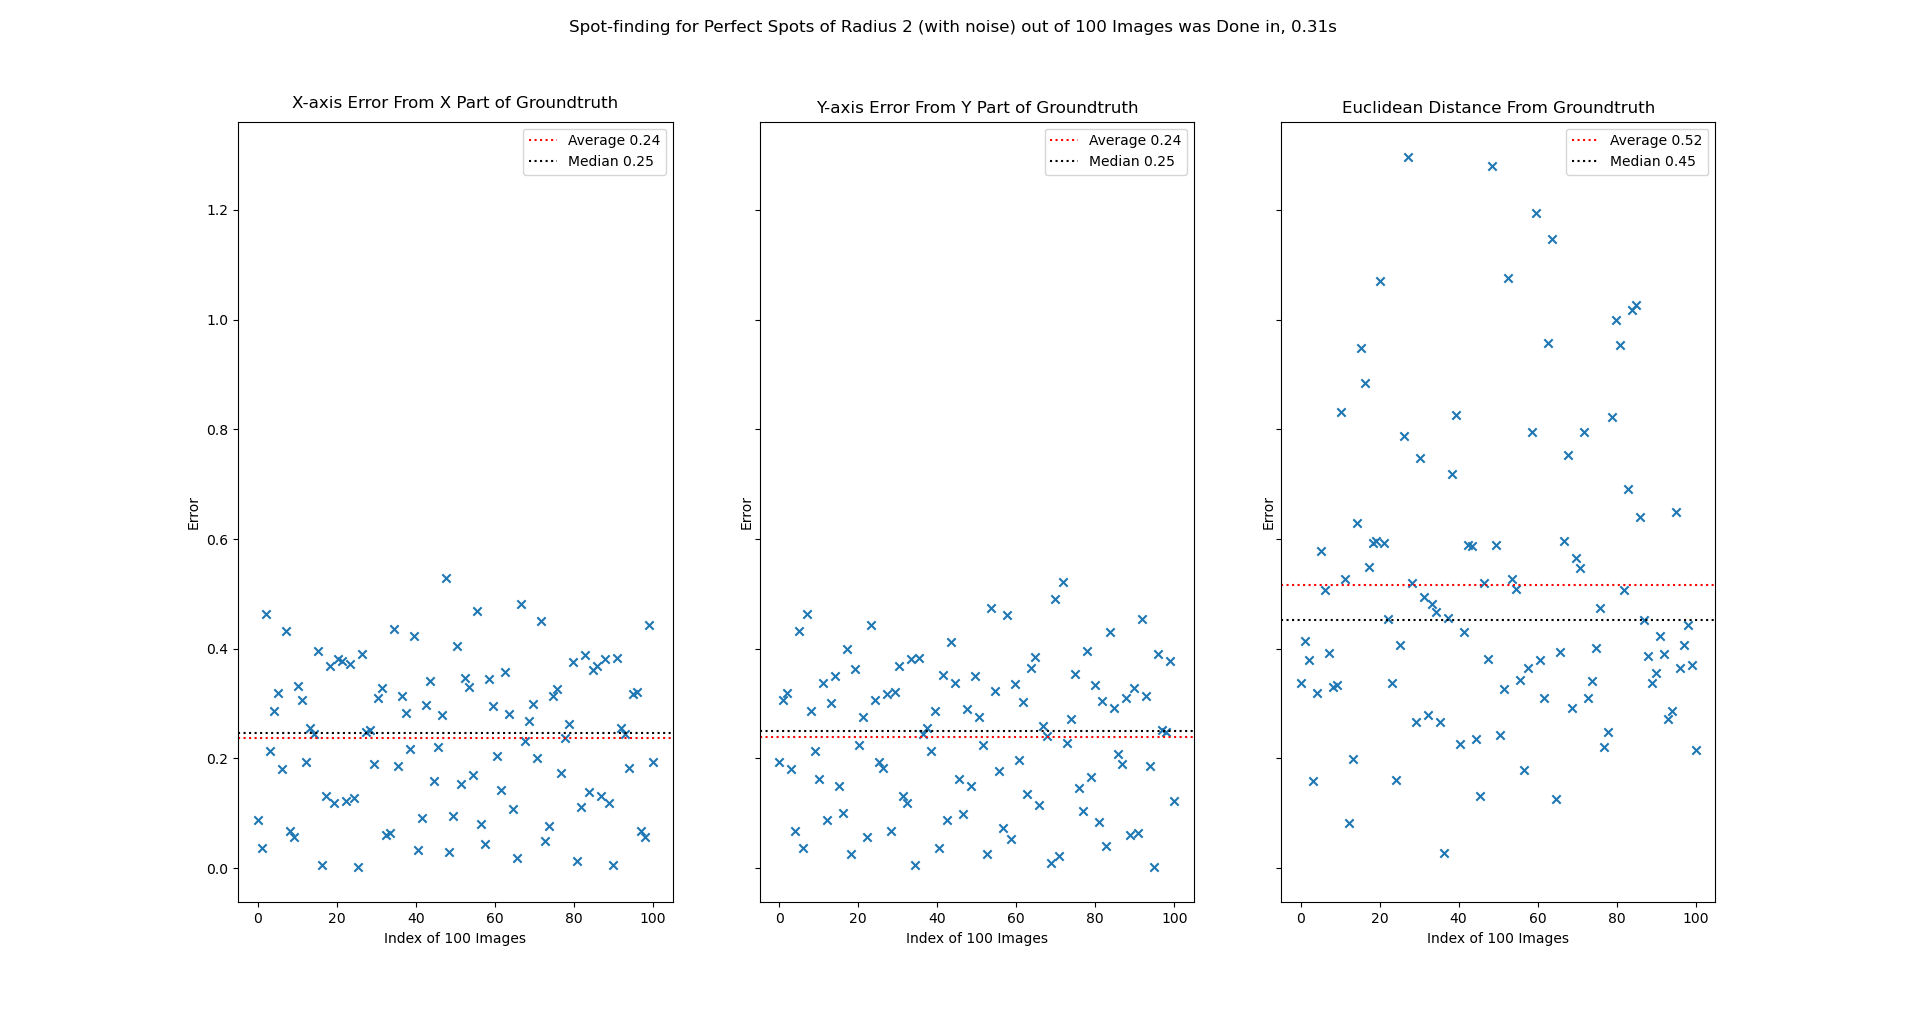
\includegraphics[width=1.0\textwidth]{project_pics/error_r2_noise.png}
      \end{center}
      \caption{}
      \label{fig:tri_er_r2_noise}
    \end{figure}
    
    \begin{figure}[H]
      \begin{center}
        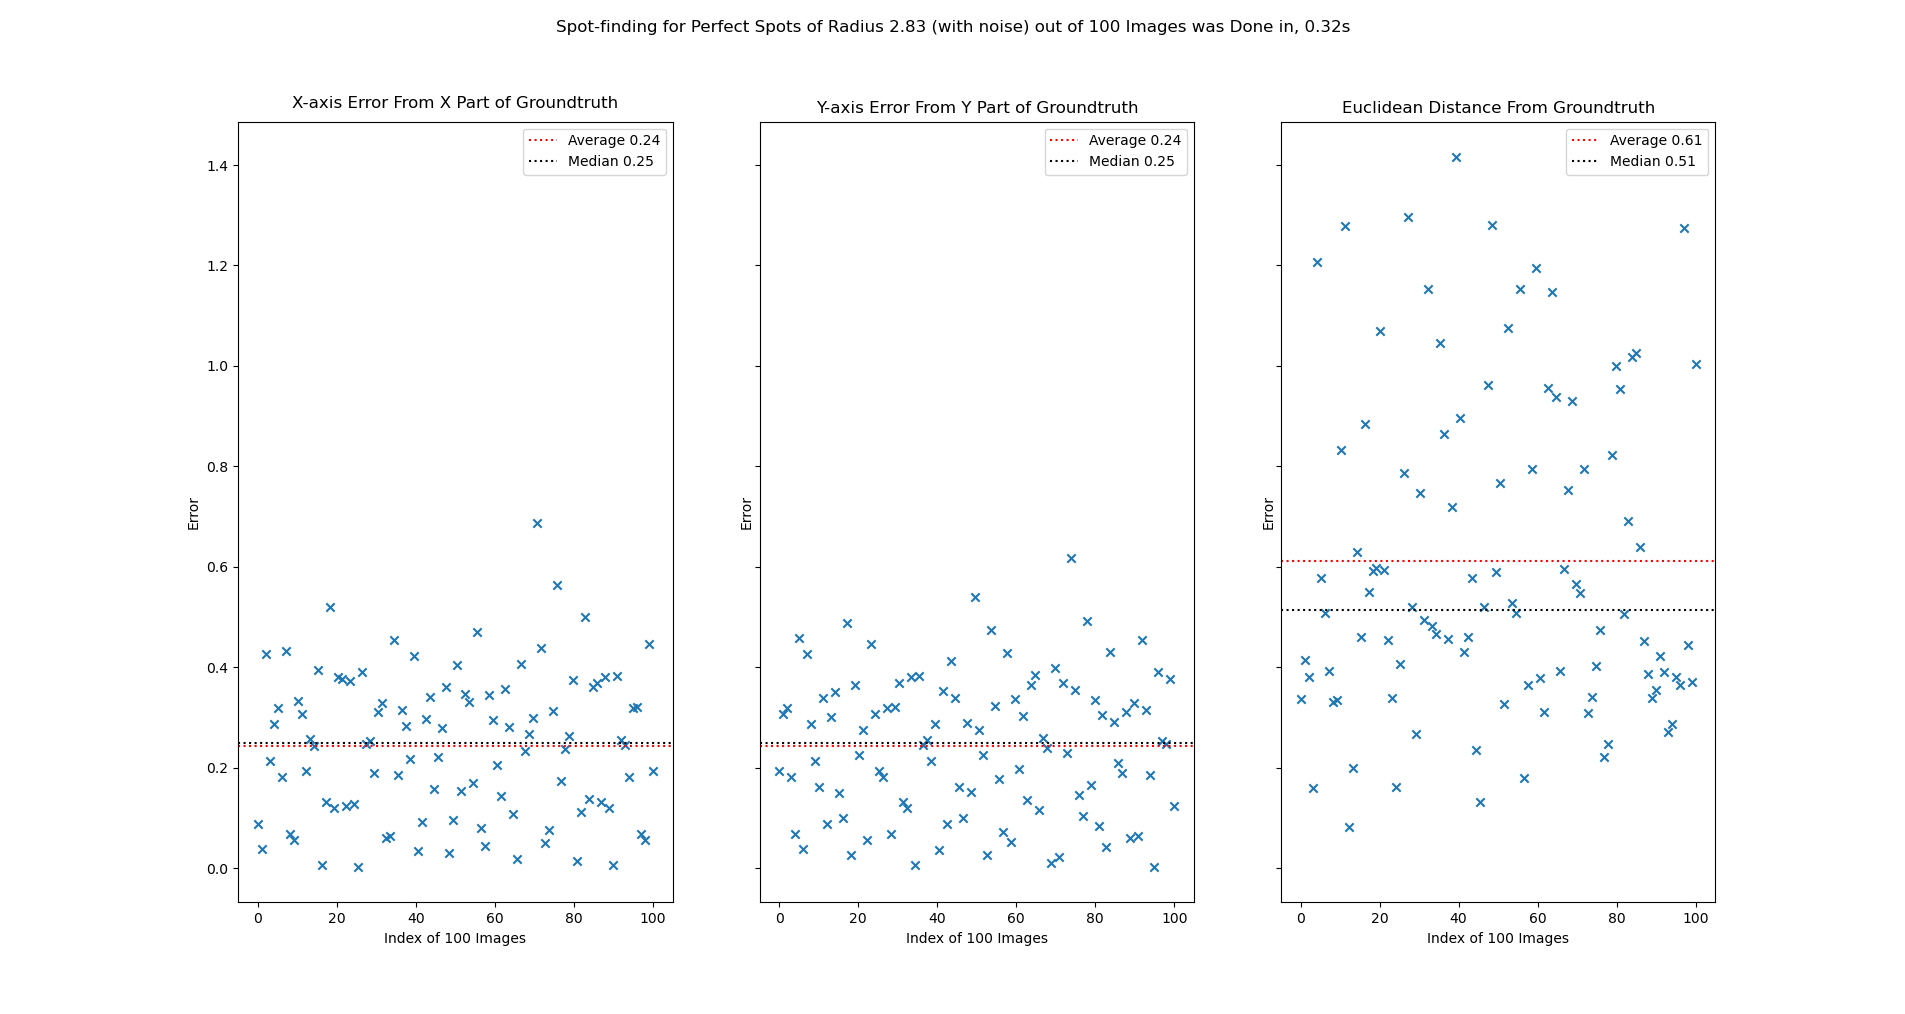
\includegraphics[width=1.0\textwidth]{project_pics/error_r283_noise.png}
      \end{center}
      \caption{}
      \label{fig:tri_er_r283_noise}
    \end{figure}
    
    \begin{figure}[H]
      \begin{center}
        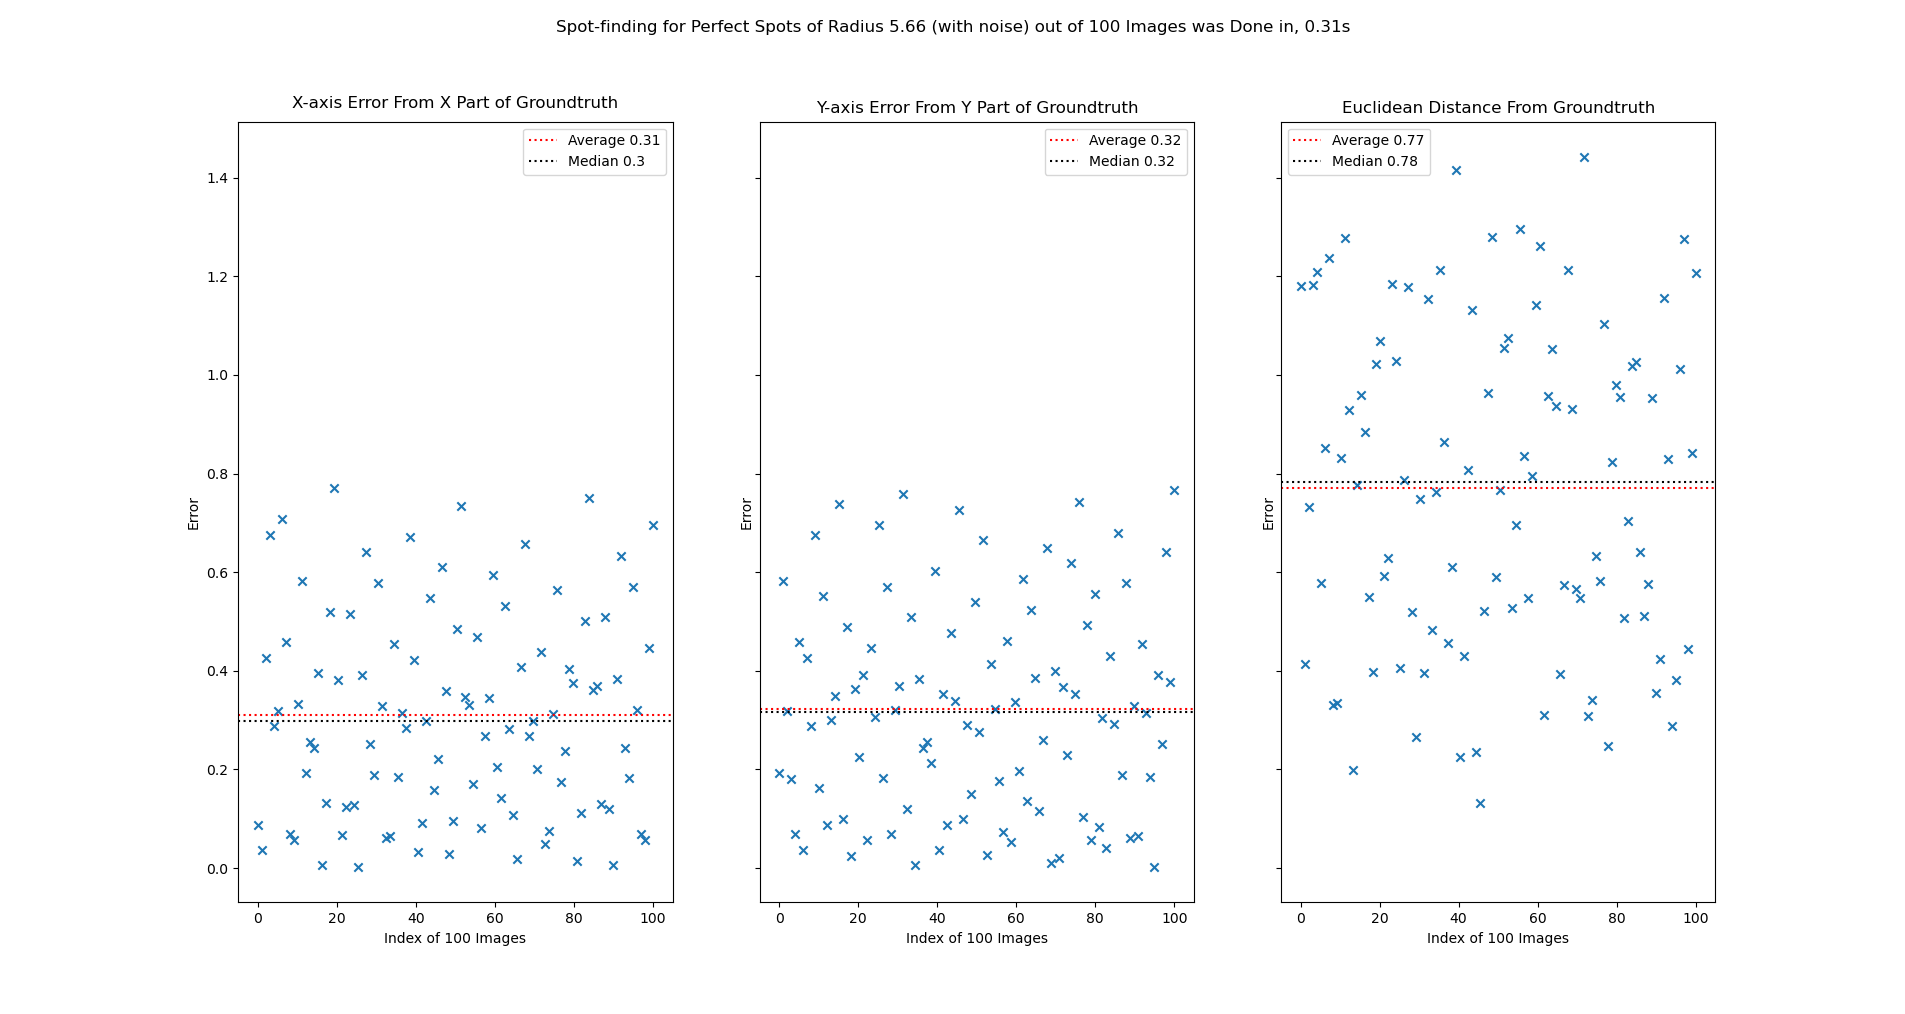
\includegraphics[width=1.0\textwidth]{project_pics/error_r566_noise.png}
      \end{center}
      \caption{}
      \label{fig:tri_er_r566_noise}
    \end{figure}
    
    \begin{figure}[H]
      \begin{center}
        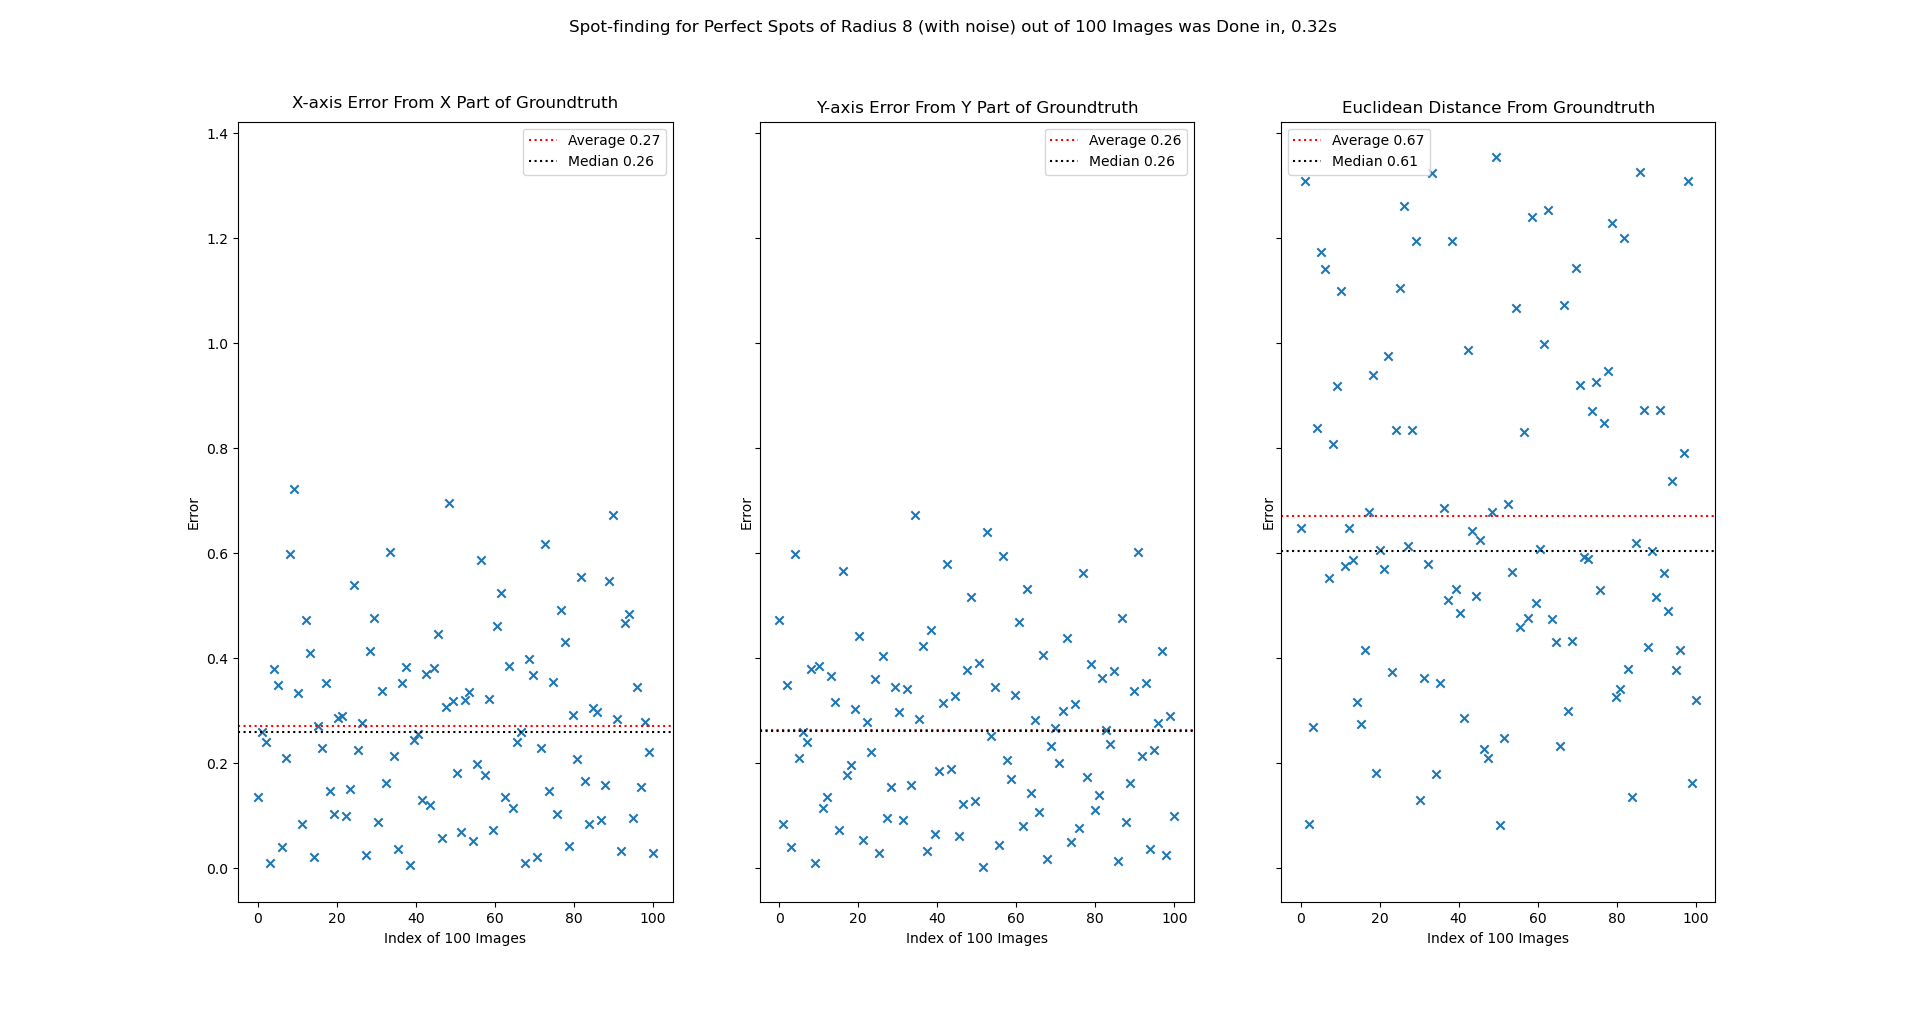
\includegraphics[width=1.0\textwidth]{project_pics/error_r8_noise.png}
      \end{center}
      \caption{}
      \label{fig:tri_er_r8_noise}
    \end{figure}
    
  
\section{Analysis (maybe don't need)}
\label{sec:Analysis}


\section{Discussion} % (fold)
\label{sec:Discussion}


  \subsection{Results in context of my aims} % (fold)
  \label{sub:Results in context of my aims}

  \subsection{Results in comparison with other studies/industry standard} % (fold)
  \label{sub:Results in comparison with other studies/industry standard}
  
  \subsection{Explanations for unexpected results} % (fold)
  \label{sub:Explanations for unexpected results}
  
  \subsection{Discuss improvements} % (fold)
  \label{sub:Discuss improvement}

% subsection subsection name (end)


\section{Conclusion} % (fold)
\label{sec:Conclusion}

% section :Conclusion (end)


\bibliographystyle{unsrt}
\bibliography{myreferences}%reads a .bib file called myreferences.bib for the actual references in BibTeX format. You can call your BibTeX file something else if you prefer.
\addcontentsline{toc}{section}{References}
%If there are problems with compiling the LaTeX file with BibTeX, make sure that file names don't have spaces in them as this might cause problems

% If there are appendices, these starts from here. Remove from this line until just before \end{document} if you are not using it 

\end{document}
